\newcommand{\usecase}[5]{{
	\setlength\extrarowheight{5pt}
	\begin{tabular}{|p{3cm}|p{10cm}|}
		\hline
		Actor & #1\\
		\hline
		Entry conditions & #2\\
		\hline
		Event flow & #3\\
		\hline
		Exit condition & #4\\
		\hline
		Exceptions & #5\\
		\hline
	\end{tabular}
}}


\chapter{Specific Requirements}

\section{Use Case Diagrams}
Here are displayed the most important use case diagrams for the various actors.

\begin{figure}[h]
\centering
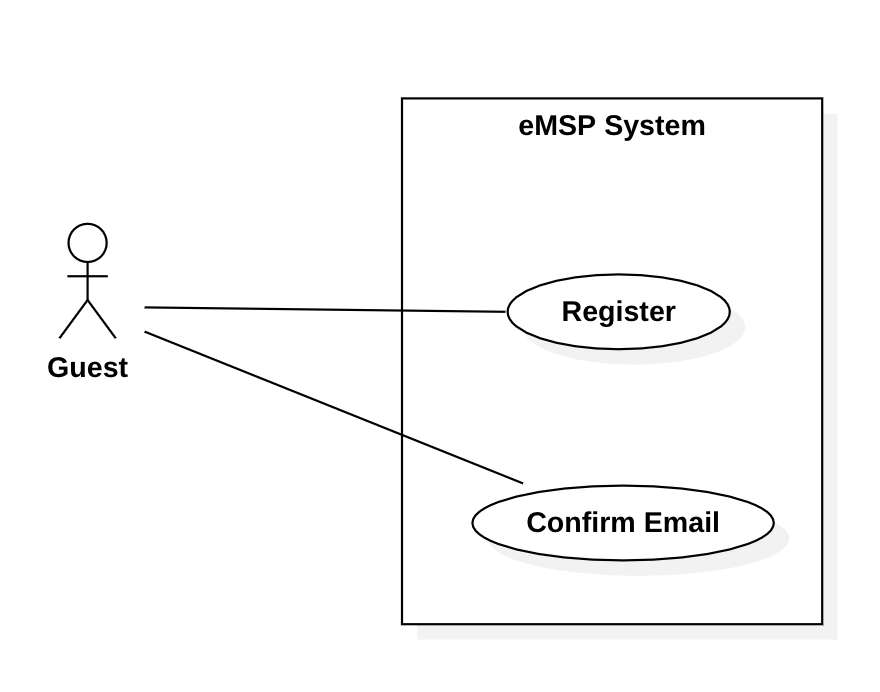
\includegraphics[width=8cm]{guest_usecase}
\caption{Use case diagram for guest user}
\end{figure}


\begin{figure}[h]
\centering
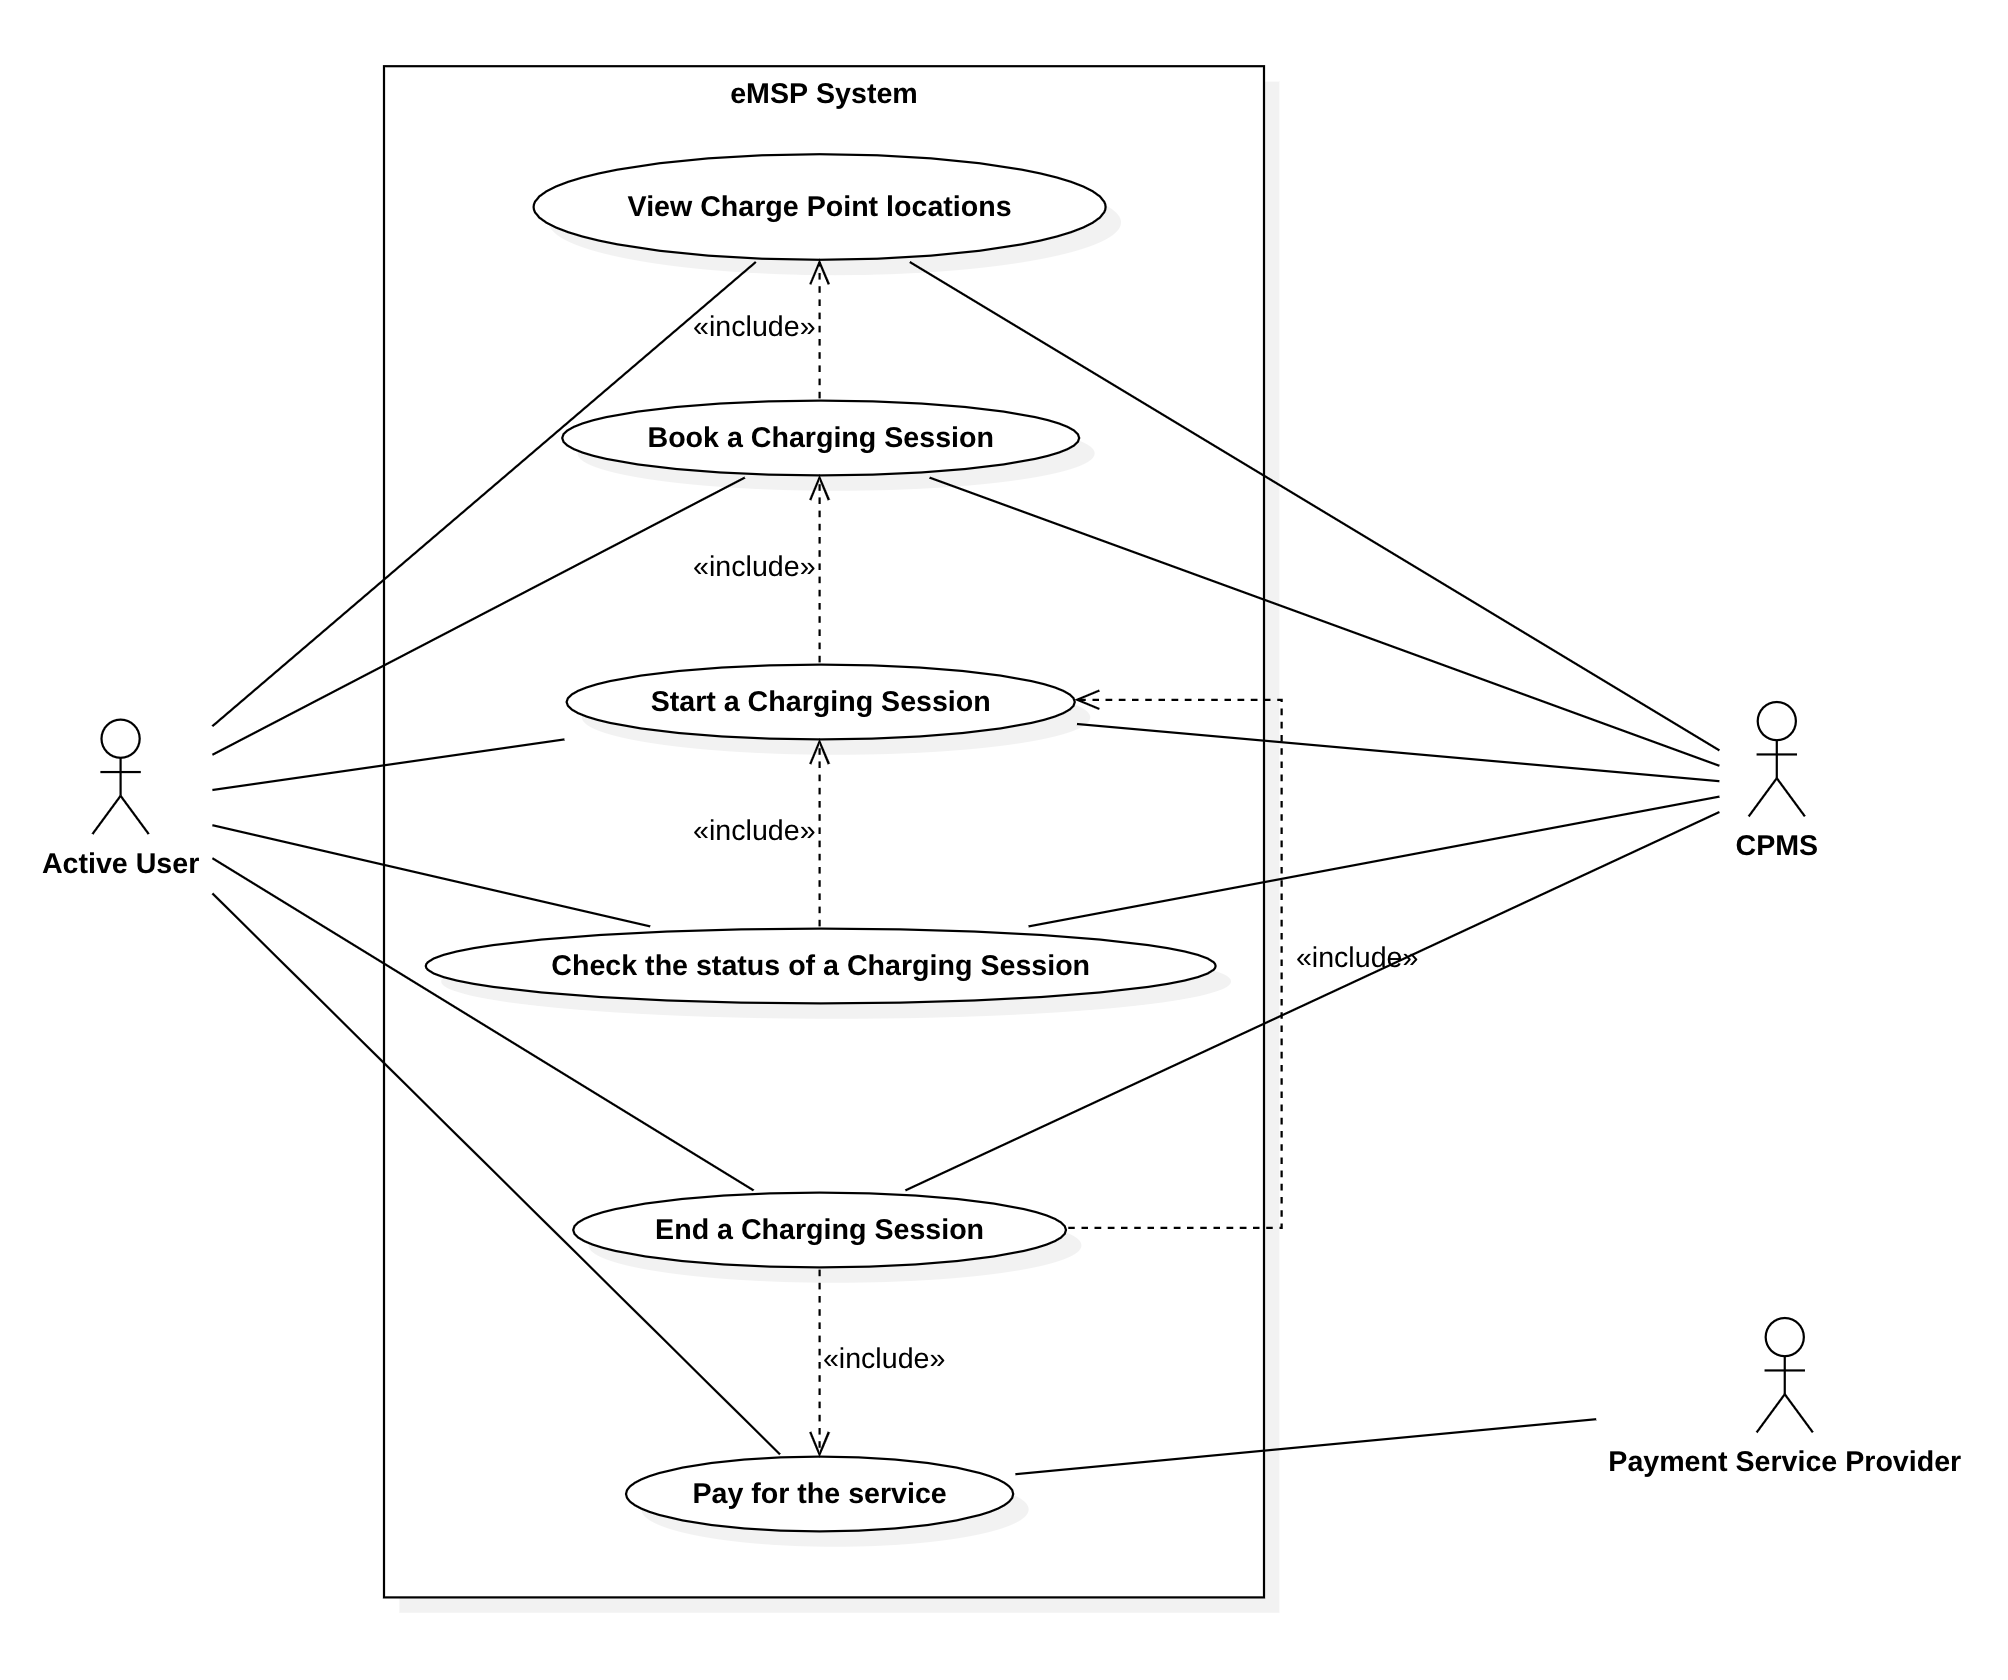
\includegraphics[width=\textwidth]{active_user_usecase}
\caption{Use case diagram for an active user and the CPMS}
\end{figure}


\begin{figure}[h]
\centering
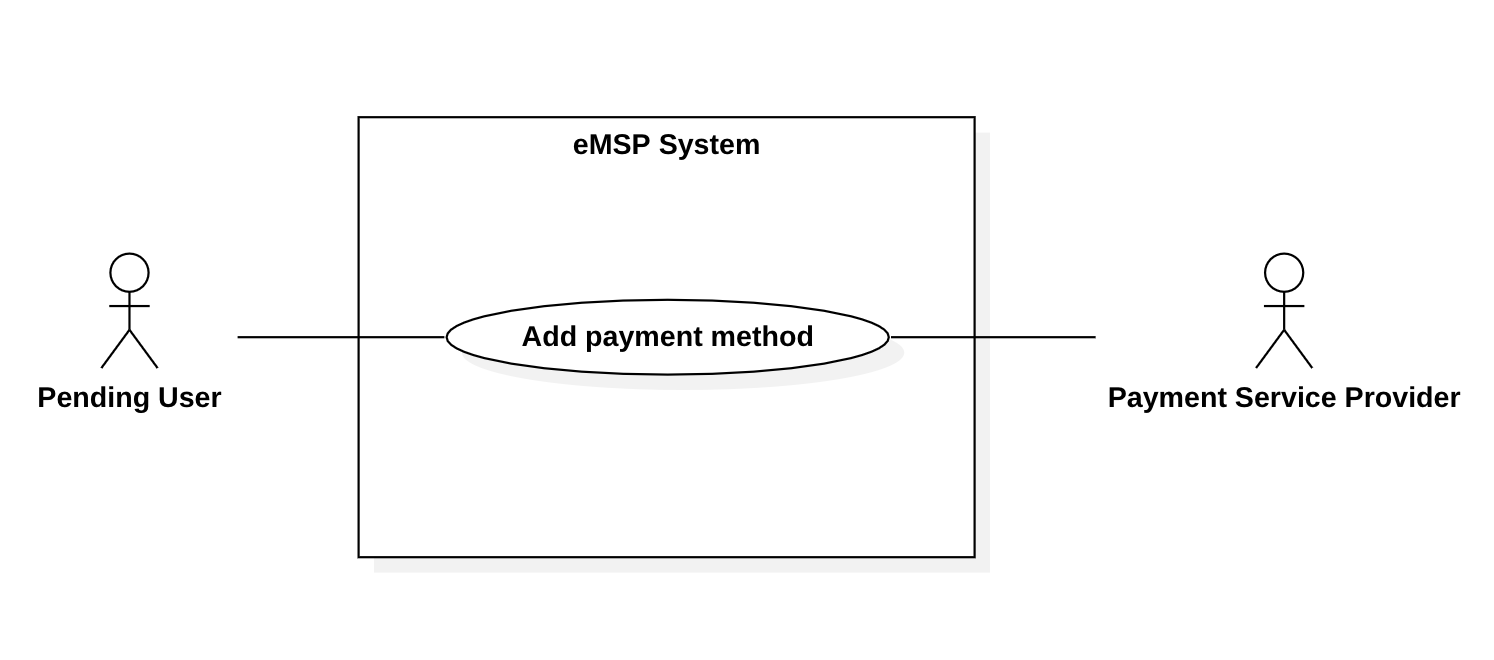
\includegraphics[width=\textwidth]{payment_provider_usecase}
\caption{Use case diagram for the Payment Service Provider and a Pending User}
\end{figure}

\clearpage


\section{Use Cases}

\begin{enumerate}
	\descitem{User registration}
	\usecase{Guest user}
	{The user is not registered to the system and is on the signup view of the mobile app}
	{
	\begin{enumerate}[1.]
	\item The guest taps on the "Signup" button
	\item The guest fills up the form
	\item The guest taps on the "Submit" button
	\item The system validates the data and create the user profile
	\item The system shows a success message and redirects the guest to the login page
	\end{enumerate}
	}
	{The user profile has been created}
	{
	\begin{enumerate}[1.]
	\item The guest does not insert all the required information
	\item The system is unavailable
	\item The system cannot process the data
	\end{enumerate}
	}
	
	
	\descitem{User login}
	\usecase{Registered user}
	{The user is registered into the system but has to log in first}
	{
	\begin{enumerate}[1.]
	\item The user taps on the "Login" button
	\item The user fills up the form
	\item The user taps on the "Submit" button
	\item The system validates the data and grants access to the user
	\item The system redirects the user to the main page
	\end{enumerate}
	}
	{The user is logged in}
	{
	\begin{enumerate}[1.]
	\item The form data are incomplete or not valid
	\item The system is unavailable
	\item The system cannot process the data
	\end{enumerate}
	}
	
	
	\descitem{View Charge Point locations}
	\usecase{Active user}
	{The user is logged in}
	{
	\begin{enumerate}[1.]
	\item The user taps on the "Explore" button
	\item The system shows a map component centred on the user location
	\item The system shows all the near Charge Point locations
	\item The user taps on a single location
	\item The system shows the details of that location to the user (e.g. availability, connector types...)
	\end{enumerate}
	}
	{The user goes to another section or closes the app}
	{
	\begin{enumerate}[1.]
	\item The system is unavailable
	\end{enumerate}
	}
	
	
	\descitem{Book a Charging session}
	\usecase{Active user}
	{The user is logged in}
	{
	\begin{enumerate}[1.]
	\item The user taps on the "Explore" button
	\item The system shows a map component centred on the user location
	\item The system shows all the near Charge Point locations
	\item The user taps on a single location
	\item The system shows the details of that location to the user (e.g. availability, connector types...)
	\item The user taps on the "Book" button
	\item The system checks the availability with the CPMS
	\item The CPMS confirms the booking to the system
	\item The system shows a confirmation message to the user with the details of the reservation
	\end{enumerate}
	}
	{The user goes to another section or closes the app}
	{
	\begin{enumerate}[1.]
	\item The system is unavailable
	\item The CPMS is unavailable or unreachable
	\item The CPMS reject the booking request
	\end{enumerate}
	}
	
	\descitem{Start a Charging session}
	\usecase{Active user}
	{The user is logged in, has an active booking and is physically at the Charging Point}
	{
	\begin{enumerate}[1.]
	\item The user taps on the "Start Charging" button
	\item The system sends the command to the CPMS
	\item The CPMS confirms the start of the charging session
	\item The system shows a confirmation message to the user
	\end{enumerate}
	}
	{The user goes to another section or closes the app}
	{
	\begin{enumerate}[1.]
	\item The system is unavailable
	\item The CPMS is unavailable or unreachable
	\item The CPMS reject the request
	\end{enumerate}
	}
	
	\descitem{User is notified about the status of the Charging session}
	\usecase{Active user and CPMS}
	{The user is logged in, has an active session and his device is connected to the internet}
	{
	\begin{enumerate}[1.]
	\item The CPMS sends a status update message to the system, informing that the Charging Session is completed
	\item The system sends a notification via the application to the user
	\item The user receives the notification
	\end{enumerate}
	}
	{A notification has been sent}
	{
	\begin{enumerate}[1.]
	\item The system is unavailable
	\item The CPMS is unavailable or unreachable
	\item The CPMS reject the request
	\item The user device is offline
	\item The user has not allowed the app to display notifications
	\end{enumerate}
	}
	
	\descitem{Complete a Charging session and pay for the service}
	\usecase{Active user, CPMS, PSP}
	{The user is logged in, has an active session and is physically at the Charing Point}
	{
	\begin{enumerate}[1.]
	\item The user taps on the "End Charging" button
	\item The system sends the command to the CPMS
	\item The CPMS confirms the end of the charging session and returns the applied tariff
	\item The system shows a success message to the user
	\item In the background the system send a request to the PSP to charge the user for the service
	\end{enumerate}
	}
	{A notification has been sent}
	{
	\begin{enumerate}[1.]
	\item The system is unavailable
	\item The CPMS is unavailable or unreachable
	\item The CPMS reject the request
	\item PSP is unavailable
	\item PSP cannot process the payment
	\end{enumerate}
	}
	
	
\end{enumerate}
\clearpage
\newpage


\section{Functional Requirements}

\section{External Interface Requirements}
\subsection{User Interfaces}
The user interface for the eMSP system is a mobile application available for both iOS and Android devices.\\
Also, as this will be a publicly available application, accessibility should be considered a priority when designing the interface.

\subsection{Hardware interfaces}
The only hardware required to use the system is a Smartphone running iOS or Android OS, with internet connection capabilities and GPS functionalities.

\subsection{Communication interfaces}
As the system needs to communicate with multiple actors, the following communication interfaces are required:

\begin{enumerate}
	\descitem{CPMS communication:}
	To share data with the various CPMS, an active, low-latency internet connection is needed.\\
   Also is required that the CPMS follows the OCPI protocol.\\
   Is important to remember that to follow the OCPI protocol, our system is required to expose a "PUSH interface" (e.g. an API endpoint that follows the protocol structure) that enables the CPMS to send newer data in real-time.
   
   \descitem{Payment Service Providers:}
    To process payments a connection with a Payment Service Provider is needed. This connection happens via proprertary API, so custom components are required to connect different providers.
\end{enumerate}


























